\section{\textit{Parameter Efficient Fine-Tuning}}

\textit{Fine-tuning} dari \textit{pre-trained model} terbukti efektif untuk berbagai tugas NLP \parencite{fine_tuning}. Namun, melakukan \textit{fine-tuning} pada seluruh model termasuk tidak efektif secara parameter karena akan menghasilkan model baru untuk setiap tugas yang dilatih. Apalagi dengan jumlah parameter yang mencapai jutaan bahkan miliaran, model yang dihasilkan dari \textit{fine-tuning} akan sangat tidak efisisen. Banyak penelitian yang mengajukan teknik \textit{fine-tuning} yang efisien secara parameter, yaitu \PEFT dengan hanya melakukan \textit{tuning} pada sebagian dari parameter model.

\subsection{\textit{Bottleneck Adapter}}

\textit{Bottleneck adapter} merupakan modul \textit{adapter} dengan menggunakan arsitektur \textit{bottleneck} \parencite{adapter_houlsby}. Konsep \textit{bottleneck adapter} diajukan sebagai alternatif dari \textit{fine-tuning}, dengan tiga properti utama, yaitu kinerja yang baik, pelatihan yang sekuensial (tidak perlu akses secara simultan terhadap keseluruhan \textit{dataset}), dan hanya menambahkan sebagain kecil parameter untuk setiap tugas \parencite{adapter_houlsby}. Strategi \textit{fine-tuning} dengan \textit{adapter} dilakukan dengan memasukkan \textit{layer} tambahan pada arsitektur \textit{Transformer} seperti yang bisa dilihat pada gambar \ref{fig:adapters_houlsby_arch}. Seperti yang telah dibahas pada subbab \ref{sec:transformer}, setiap \textit{layer} pada \textit{Transformer} mempunyai dua \textit{sub-layer}, yaitu \textit{multi-head attention} dan \textit{feed-forward}. Metode \textit{bottleneck adapter} ini akan menambahkan modul \textit{adapter} ke setiap \textit{sub-layer} pada \textit{Transformer} tersebut \parencite{adapter_houlsby}.

\begin{figure}[h]
    \vspace{0.25cm}
    \centering
    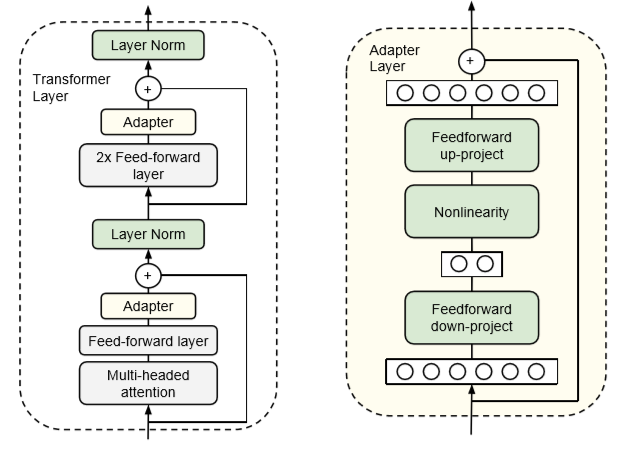
\includegraphics[width=\textwidth]{chapter-2/adapter_houlsby_arch.png}
    \caption{Arsitektur dari \textit{Bottleneck Adapter} oleh \citeauthor{adapter_houlsby} \parencite{adapter_houlsby}}
    \label{fig:adapters_houlsby_arch}
\end{figure}

Arsitektur \textit{bottleneck} dari modul \textit{adapter} diajukan untuk membatasi jumlah dari parameter \parencite{adapter_houlsby}. Berdasarkan gambar \ref{fig:adapters_houlsby_arch}, \textit{adapter} melakukan proyeksi dari dimensi asli $d$ ke dimensi yang lebih kecil $m$, lalu dilanjutkan dengan fungsi nonlinear, dan dilakukan proyeksi kembali dari dimensi $m$ ke dimensi asli $d$. Sehingga, total parameter yang ditambahkan untuk setiap \textit{layer} adalah $2md$ yang berasal dari bobot pada kedua proyeksi ditambah dengan $m+d$ yang merupakan biasnya. Pada penggunaannya, dengan memakai nilai $m << d$, parameter yang digunakan adalah sekitar $0.5-8\%$ dari parameter asli model \parencite{adapter_houlsby}.

\begin{equation}
    reduction\_factor = \frac{d_{hidden}}{d_{bottleneck}}
    \label{eq:reduction_factor}
\end{equation}

Parameter yang digunakan dibatasi dengan menggunakan $reduction\_factor$ \parencite{adapterhub}. Nilai dari $reduction\_factor$ tersebut didapat dari rasio antara dimensi asli dengan dimensi yang lebih kecil bisa dilihat pada rumus \ref{eq:reduction_factor} \parencite{adapterhub}. Nilai $d_{hidden}$ merupakan nilai dari dimensi asli $d$. Sedangkan, nilai $d_{bottleneck}$ merupakan dimensi dari \textit{bottleneck} yang lebih kecil dari dimensi aslinya.

Penggunaan \textit{adapter} tidak hanya dengan menambahkannya pada setiap \textit{sub-layer Transformer}. Terdapat beberapa konfigurasi yang bisa digunakan. Salah satunya adalah seperti pada gambar \ref{fig:adapters_houlsby_arch} oleh \parencite{adapter_houlsby} dengan menambahkan modul \textit{adapter} pada kedua \textit{sub-layer} (\textit{multi-head attention} dan \textit{feed-forward}). \parencite{adapter_pfeiffer} menggunakan \textit{adapter} hanya pada \textit{sub-layer feed-forward}. Sedangkan, \citeauthor{uvpl} menggunakan \textit{adapter} secara paralel pada \textit{layer transformer}.

\subsection{\textit{Low Rank Adaptation} (LoRA)}

Konsep dasar di balik LoRA adalah ide bahwa adaptasi model untuk tugas baru tidak selalu memerlukan perubahan besar pada seluruh parameter model. Sebaliknya, perubahan kecil pada representasi tertentu dapat menghasilkan peningkatan kinerja yang signifikan. Dengan fokus pada \textit{low rank adaptation}, LoRA mengubah hanya sebagian kecil dari bobot model, sementara sebagian besar bobot lainnya tetap tidak berubah. Ini berarti bahwa hanya "sebagian" dari informasi dalam model yang diperbarui, yang mengarah pada efisiensi komputasi yang meningkat \parencite{lora}.

\begin{figure}[h]
    \vspace{0.25cm}
    \centering
    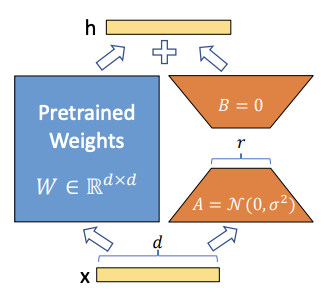
\includegraphics[width=0.8\textwidth]{chapter-2/lora.png}
    \caption{Arsitektur LoRA \parencite{lora}}
    \label{fig:lora}
\end{figure}

Salah satu kelebihan utama dari pendekatan ini adalah kemampuannya untuk mengurangi \textit{overhead} komputasi. Dalam praktiknya, ini berarti waktu \textit{training} dan sumber daya yang diperlukan untuk adaptasi model menjadi jauh lebih sedikit dibandingkan dengan metode lain yang mungkin melibatkan \textit{training} ulang model dari awal atau menambahkan sejumlah besar parameter tambahan. Arsitektur dari LoRA dapat dilihat pada Gambar \ref{fig:lora}.

Pendekatan LoRA menjadi sangat relevan, terutama saat berhadapan dengan model-model berukuran besar. Model-model seperti ini memiliki jumlah parameter yang sangat besar, sehingga \textit{training} ulang atau menambahkan parameter tambahan bisa menjadi sangat mahal dari segi komputasi. Dengan LoRA, adaptasi model-model besar menjadi lebih praktis dan dapat dilakukan dengan efisiensi yang jauh lebih tinggi, tanpa mengorbankan kinerja. Dengan demikian, LoRA menawarkan pendekatan yang menjanjikan untuk mengadaptasi \textit{pre-trained model} dengan cara yang lebih efisien.

\subsection{\textit{Prefix-Tuning}}

\textit{Prefix-Tuning} adalah teknik yang diperkenalkan untuk mengoptimalkan \textit{prompt} kontinu dalam generasi teks. Berbeda dengan pendekatan  yang melibatkan \textit{training} ulang seluruh model atau menambahkan parameter tambahan, \textit{Prefix-Tuning} fokus pada pengoptimalan sejumlah kecil parameter yang didefinisikan sebagai "prefix" dari sekuens input \parencite{prefix_tuning} Dengan kata lain, dibanding mengubah seluruh model, hanya \textit{prefix-tuning} dari input yang dioptimalkan untuk meningkatkan kinerja generasi dengan arsitekturnya dapat dilihat pada Gambar \ref{fig:prefix-tuning}.

\begin{figure}[h]
    \vspace{0.25cm}
    \centering
    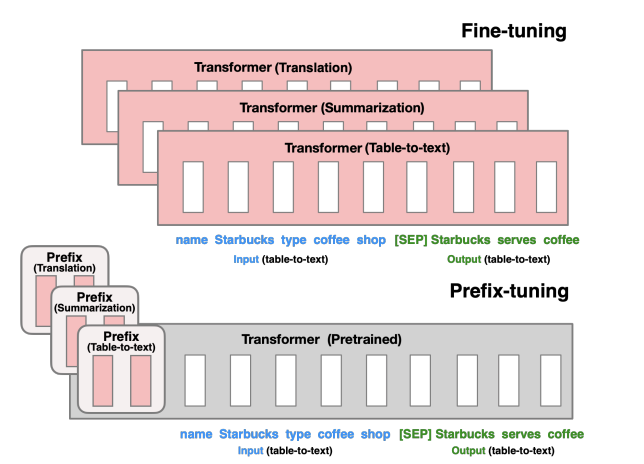
\includegraphics[width=0.8\textwidth]{chapter-2/prefix-tuning.png}
    \caption{Arsitektur \textit{Prefix-Tuning} \parencite{prefix_tuning}}
    \label{fig:prefix-tuning}
\end{figure}

Keuntungan utama dari pendekatan ini adalah efisiensi. Dengan mengoptimalkan hanya sebagian kecil dari parameter, \textit{Prefix-Tuning} dapat mencapai peningkatan kinerja dengan \textit{overhead} komputasi yang jauh lebih rendah dibandingkan dengan teknik \textit{fine-tuning} . Selain itu, dengan fokus pada \textit{prefix}, teknik ini memungkinkan adaptasi yang lebih spesifik terhadap tugas atau domain tertentu, memberikan fleksibilitas lebih dalam aplikasi praktis.

Teknik ini dapat digunakan untuk meningkatkan kinerja model generatif di berbagai tugas, termasuk penerjemahan mesin, peringkasan teks, dan lainnya. Hasil eksperimen menunjukkan bahwa \textit{Prefix-Tuning} mampu mencapai kinerja yang sebanding atau bahkan lebih baik dibandingkan dengan metode \textit{fine-tuning} , tetapi dengan biaya komputasi yang jauh lebih rendah.

